\documentclass[conference]{IEEEtran}
\IEEEoverridecommandlockouts
\newcommand{\BIBTeX}{BIB\TeX}

\usepackage{cite}
\usepackage{amsmath,amssymb,amsfonts}
\usepackage{algorithmic}
\usepackage{graphicx}
\usepackage{textcomp}
\usepackage{xcolor}
\usepackage{booktabs}
\usepackage{multirow}
\usepackage{hyperref}
\usepackage{cleveref}
\usepackage{subcaption}
\usepackage{tikz}
\usetikzlibrary{positioning, arrows.meta, shapes.geometric, fit, calc, backgrounds, decorations.pathreplacing}

\def\BibTeX{{\rm B\kern-.05em{\sc i\kern-.025em b}\kern-.08emT\kern-.1667em\lower.7ex\hbox{E}\kern-.125emX}}

\begin{document}

\title{WaveLKCell: Multi-Level Wavelet Enhancement for Large-Kernel Cell Nuclei Instance Segmentation}

\author{
\IEEEauthorblockN{
    % TODO: Add author names
    First Author\IEEEauthorrefmark{1},
    Second Author\IEEEauthorrefmark{1}
}
\IEEEauthorblockA{
    \IEEEauthorrefmark{1}Department of Electrical and Information Engineering,
    Universitas Gadjah Mada, Yogyakarta, Indonesia\\
    % TODO: Add email
}
}

\maketitle

\begin{abstract}
% TODO: Fill in final numbers after training
Accurate cell nuclei instance segmentation in hematoxylin and eosin (H\&E) stained tissue images is essential for computational pathology. Recent large-kernel convolutional methods such as LKCell achieve state-of-the-art performance with efficient computation by expanding the receptive field through large convolution kernels. However, large kernels may blur fine high-frequency details critical for delineating nuclear boundaries and capturing chromatin texture. In this paper, we propose WaveLKCell, which integrates a multi-level wavelet enhancement module into the large-kernel segmentation framework. Our approach applies two-level Haar discrete wavelet transform (DWT) to the deepest encoder features, decomposing them into frequency sub-bands that are processed by specialized modules: Adaptive Power Gabor Convolution (APGConv) for high-frequency boundary details, self-attention for mid-high frequencies, channel attention for mid-low frequencies, and depthwise convolution for low frequencies. The enhanced features are reconstructed via inverse DWT with a residual connection and fed to a large-kernel decoder for nuclei prediction. Experiments on the PanNuke benchmark demonstrate that WaveLKCell achieves competitive performance, achieving an mPQ of \textbf{[X.XXXX]} and a bPQ of \textbf{[X.XXXX]}, validating the benefit of wavelet-enhanced frequency decomposition for large-kernel nuclei segmentation.
\end{abstract}

\begin{IEEEkeywords}
nuclei instance segmentation, wavelet transform, large convolution kernel, computational pathology, frequency decomposition
\end{IEEEkeywords}

%% ============================================================
\section{Introduction}
\label{sec:intro}
%% ============================================================

Cell nuclei instance segmentation in hematoxylin and eosin (H\&E) stained tissue images is a fundamental task in computational pathology, enabling quantitative analysis of tumor cell density, nucleus-to-cytoplasm ratio, and nuclear morphology for cancer grading and prognosis~\cite{lkcell}. With the rapid development of deep learning, automated nuclei segmentation methods have emerged as powerful tools to reduce the burden on healthcare systems.

Despite significant progress, achieving high-performance and efficient nuclei segmentation remains challenging due to uneven staining, cell overlap, and clustered morphology. Previous convolutional neural network (CNN)-based methods~\cite{hoevernet, stardist, micro_net} employ U-shaped architectures with small convolution kernels (typically $3{\times}3$) that limit the receptive field. While Vision Transformer (ViT)-based methods~\cite{cellvit, swin_unet} introduce global receptive fields, they incur substantial computational costs that hinder clinical deployment.

LKCell~\cite{lkcell} addresses this trade-off by introducing large convolution kernels into nuclei segmentation for the first time, achieving state-of-the-art results with only 21.6\% of the FLOPs compared to the previous leading method. However, large-kernel convolutions inherently apply spatial averaging over their receptive field, which can attenuate high-frequency information such as nuclear boundaries and fine chromatin patterns. These high-frequency details are precisely the cues needed for accurate instance separation and type classification.

To address this limitation, we draw inspiration from wavelet-based image analysis, which provides a principled framework for decomposing signals into frequency sub-bands. WaveConvX~\cite{waveconvx} recently demonstrated that multi-level wavelet enhancement with frequency-specific processing significantly improves histopathology image classification. This motivates the question: \emph{can wavelet-based frequency decomposition complement large-kernel convolutions for nuclei segmentation?}

In this paper, we propose WaveLKCell, a method that integrates multi-level wavelet enhancement into the large-kernel nuclei segmentation framework. Our key insight is that wavelet decomposition and large-kernel convolutions operate on complementary frequency domains---large kernels capture broad spatial context in the low-frequency regime, while wavelet processing explicitly recovers and enhances the high-frequency details that large kernels tend to blur. Specifically, our contributions are:

\begin{itemize}
    \item We propose WaveLKCell, which integrates a two-level Haar wavelet enhancement module into a large-kernel encoder-decoder architecture for cell nuclei instance segmentation.
    \item We employ frequency-specific processors---Adaptive Power Gabor Convolution (APGConv) for high-frequency nuclear boundaries, self-attention for mid-high frequencies, channel attention for mid-low frequencies, and depthwise convolution for low frequencies---to selectively enhance the features most relevant to nuclei segmentation.
    \item Experiments on the PanNuke dataset demonstrate competitive performance against state-of-the-art methods including CellPose-SAM, StarDist, LSP-DETR, and LKCell.
\end{itemize}

%% ============================================================
\section{Related Work}
\label{sec:related}
%% ============================================================

\subsection{Nuclei Instance Segmentation}

Traditional image processing techniques for nuclei segmentation rely on hand-crafted features and domain knowledge. The watershed algorithm~\cite{watershed} separates clustered nuclei using marker-controlled flooding, while approaches based on nuclear geometry require careful parameter tuning. These methods are inherently limited in representational capacity.

Deep learning has become the dominant paradigm. U-Net~\cite{unet} established the encoder-decoder architecture with skip connections that has become the standard for medical image segmentation. HoVerNet~\cite{hoevernet} introduced the horizontal-vertical (HV) map representation alongside nuclear pixel (NP) and nuclear type (NT) predictions, using three separate decoder branches. CPP-Net~\cite{cppnet} added parallel convolution layers for post-processing. StarDist~\cite{stardist} represents nuclei as star-convex polygons for instance separation. CellPose~\cite{cellpose} uses gradient fields for cell boundary detection, and recent CellPose-SAM variants leverage foundation model features. LSP-DETR~\cite{lsp_detr} adapts detection transformers for nuclei segmentation.

LKCell~\cite{lkcell} demonstrated that large convolution kernels, previously successful in natural image analysis~\cite{replknet, unireplknet}, can achieve state-of-the-art nuclei segmentation with significantly reduced computation. However, large kernels may not optimally preserve high-frequency boundary details.

\subsection{Wavelet Transforms in Medical Imaging}

Wavelet transforms decompose signals into localized frequency sub-bands, enabling multi-resolution analysis. In medical imaging, wavelets have been used for denoising, feature extraction, and texture analysis. Recent works have integrated wavelets into deep learning pipelines. WaveMix~\cite{wavemix} uses wavelet-based token mixing for image classification. WaveConvX~\cite{waveconvx} proposed multi-level wavelet enhancement within ConvNeXt for histopathology classification, demonstrating that frequency-specific processing improves feature representation.

Our work extends this idea from classification to instance segmentation, and specifically targets the complementary relationship between large-kernel convolutions and wavelet frequency decomposition.

%% ============================================================
\section{Methodology}
\label{sec:method}
%% ============================================================

\subsection{Overview}

As illustrated in \cref{fig:architecture}, WaveLKCell consists of four main components: (1) a large-kernel encoder based on the UniRepLKNet architecture~\cite{unireplknet}, (2) a multi-level wavelet enhancement module that processes the deepest encoder features, (3) a large-kernel decoder with skip connections, and (4) segmentation and classification heads.

Given an input H\&E image $\mathbf{X} \in \mathbb{R}^{3 \times H \times W}$, the encoder extracts multi-scale features $\{\mathbf{F}_1, \mathbf{F}_2, \mathbf{F}_3\}$ at three stages with dimensions $\{96, 192, 384\}$ and spatial resolutions $\{H/4, H/8, H/16\}$. The deepest features $\mathbf{F}_3$ are enhanced by the wavelet module to produce $\tilde{\mathbf{F}}_3$, which is then downsampled to $\mathbf{F}_4 \in \mathbb{R}^{768 \times H/32 \times W/32}$ for the decoder bottleneck.

The decoder progressively upsamples features through three large-kernel decoder blocks with skip connections from $\mathbf{F}_3$, $\mathbf{F}_2$, and $\mathbf{F}_1$, followed by two additional upsampling stages that incorporate early input features. Three segmentation heads predict the nuclear pixel (NP) binary map, horizontal-vertical (HV) map, and nuclear type (NT) map.

\begin{figure*}[t]
\centering
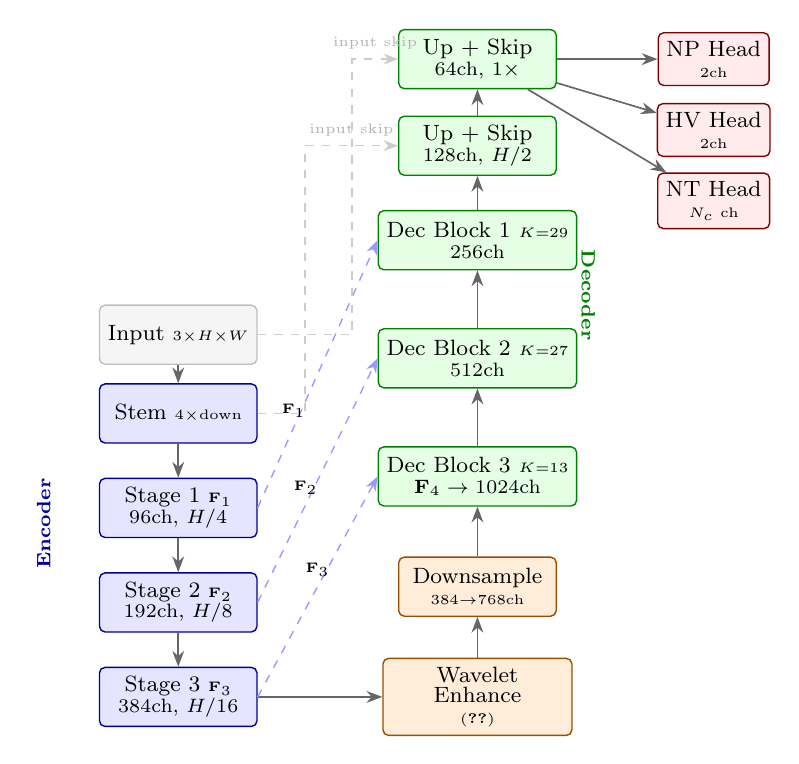
\begin{tikzpicture}[
    >=Stealth,
    block/.style={
        draw, rounded corners=2pt, minimum height=0.75cm, minimum width=2.0cm,
        font=\footnotesize, align=center, line width=0.5pt, inner sep=3pt
    },
    enc/.style={block, fill=blue!10, draw=blue!60!black},
    wav/.style={block, fill=orange!15, draw=orange!60!black},
    dec/.style={block, fill=green!10, draw=green!50!black},
    head/.style={block, fill=red!8, draw=red!50!black, minimum width=1.2cm, minimum height=0.65cm},
    aux/.style={block, fill=yellow!15, draw=yellow!60!black},
    arr/.style={->, draw=black!60, line width=0.6pt},
    skip/.style={->, draw=blue!40, dashed, line width=0.5pt},
]

% ====== ENCODER (left, going DOWN) ======
\node[block, fill=gray!8, draw=gray!50] (input) at (0, 0) {Input {\tiny $3{\times}H{\times}W$}};

\node[enc] (stem) at (0, -1.0) {Stem {\tiny $4{\times}$down}};

\node[enc] (s1) at (0, -2.2) {Stage 1 {\tiny $\mathbf{F}_1$}\\[-2pt]{\scriptsize 96ch, $H/4$}};

\node[enc] (s2) at (0, -3.4) {Stage 2 {\tiny $\mathbf{F}_2$}\\[-2pt]{\scriptsize 192ch, $H/8$}};

\node[enc] (s3) at (0, -4.6) {Stage 3 {\tiny $\mathbf{F}_3$}\\[-2pt]{\scriptsize 384ch, $H/16$}};

% ====== BOTTLENECK (bottom center) ======
\node[wav, minimum width=2.4cm] (we) at (3.8, -4.6) {Wavelet\\[-2pt]Enhance\\[-2pt]{\tiny(\cref{fig:wavelet})}};

\node[wav, minimum width=2.0cm] (ds) at (3.8, -3.2) {Downsample\\[-2pt]{\tiny $384{\to}768$ch}};

% ====== DECODER (right, going UP) ======
\node[dec] (d3) at (3.8, -1.8) {Dec Block 3 {\tiny $K{=}13$}\\[-2pt]{\scriptsize $\mathbf{F}_4 \to 1024$ch}};

\node[dec] (d2) at (3.8, -0.3) {Dec Block 2 {\tiny $K{=}27$}\\[-2pt]{\scriptsize $512$ch}};

\node[dec] (d1) at (3.8, 1.2) {Dec Block 1 {\tiny $K{=}29$}\\[-2pt]{\scriptsize $256$ch}};

\node[dec] (up2) at (3.8, 2.4) {Up $+$ Skip\\[-2pt]{\scriptsize $128$ch, $H/2$}};

\node[dec] (up1) at (3.8, 3.5) {Up $+$ Skip\\[-2pt]{\scriptsize $64$ch, $1{\times}$}};

% ====== HEADS (top right) ======
\node[head] (np) at (6.8, 3.5) {NP Head\\[-2pt]{\tiny 2ch}};
\node[head] (hv) at (6.8, 2.6) {HV Head\\[-2pt]{\tiny 2ch}};
\node[head] (nt) at (6.8, 1.7) {NT Head\\[-2pt]{\tiny $N_c$ ch}};

% ====== MAIN FLOW (encoder down) ======
\draw[arr] (input) -- (stem);
\draw[arr] (stem) -- (s1);
\draw[arr] (s1) -- (s2);
\draw[arr] (s2) -- (s3);

% Encoder -> Wavelet -> Downsample (bottom, going right then up)
\draw[arr] (s3) -- (we);
\draw[arr] (we) -- (ds);

% Downsample -> Decoder (going up)
\draw[arr] (ds) -- (d3);
\draw[arr] (d3) -- (d2);
\draw[arr] (d2) -- (d1);
\draw[arr] (d1) -- (up2);
\draw[arr] (up2) -- (up1);

% Heads
\draw[arr] (up1) -- (np);
\draw[arr] (up1) -- (hv);
\draw[arr] (up1) -- (nt);

% ====== SKIP CONNECTIONS (horizontal, encoder to decoder) ======
\draw[skip] (s3.east) -- node[above, font=\tiny] {$\mathbf{F}_3$} (d3.west);
\draw[skip] (s2.east) -- node[above, font=\tiny, pos=0.4] {$\mathbf{F}_2$} (d2.west);
\draw[skip] (s1.east) -- node[above, font=\tiny, pos=0.3] {$\mathbf{F}_1$} (d1.west);

% Input feature skips to extra upsampling
\draw[skip, draw=gray!40] (stem.east) -- ++(0.6,0) |- node[near end, above, font=\tiny, text=gray!60] {input skip} (up2.west);
\draw[skip, draw=gray!40] (input.east) -- ++(1.2,0) |- node[near end, above, font=\tiny, text=gray!60] {input skip} (up1.west);

% ====== ANNOTATIONS ======
\node[font=\scriptsize\bfseries, text=blue!60!black, rotate=90, anchor=south] at (-1.5, -2.4) {Encoder};
\node[font=\scriptsize\bfseries, text=green!50!black, rotate=-90, anchor=south] at (5.0, 0.5) {Decoder};

\end{tikzpicture}
\caption{Overview of the WaveLKCell architecture in a U-shaped encoder-decoder layout. The large-kernel encoder (UniRepLKNet-S) extracts multi-scale features $\{\mathbf{F}_1, \mathbf{F}_2, \mathbf{F}_3\}$ at progressively lower resolutions. The Multi-Level Wavelet Enhancement module processes $\mathbf{F}_3$ through two-level Haar DWT/IDWT with frequency-specific processors (\cref{fig:wavelet}), producing the bottleneck $\mathbf{F}_4$. The decoder upsamples through three large-kernel blocks with skip connections (dashed blue), followed by two extra upsampling stages. Three heads predict NP, HV, and NT maps.}
\label{fig:architecture}
\end{figure*}

\begin{figure}[t]
\centering
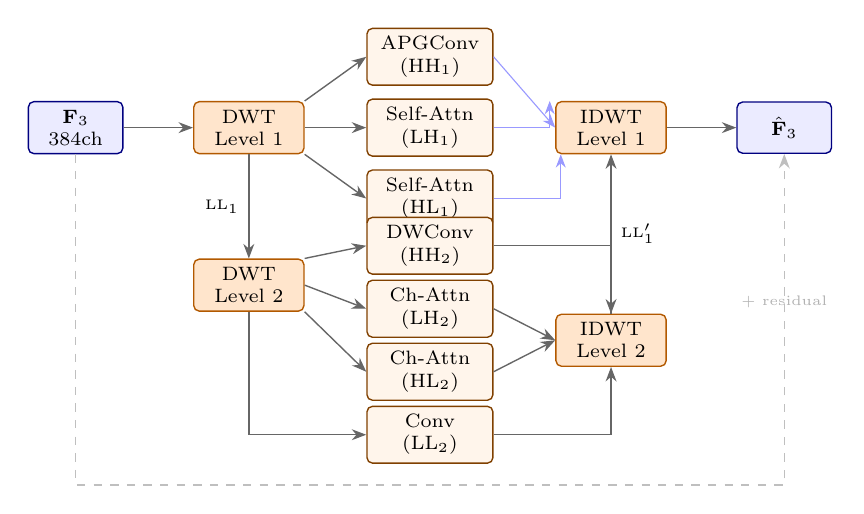
\begin{tikzpicture}[
    >=Stealth,
    block/.style={
        draw, rounded corners=2pt, minimum height=0.65cm,
        font=\scriptsize, align=center, line width=0.5pt, inner sep=3pt
    },
    dwt/.style={block, fill=orange!20, draw=orange!70!black, minimum width=1.4cm},
    proc/.style={block, fill=orange!8, draw=orange!50!black, minimum width=1.6cm},
    idwt/.style={block, fill=orange!20, draw=orange!70!black, minimum width=1.4cm},
    arr/.style={->, draw=black!60, line width=0.5pt},
    skiparr/.style={->, draw=blue!40, line width=0.4pt},
]

% Input
\node[block, fill=blue!8, draw=blue!50!black, minimum width=1.2cm] (fin) at (0,0) {$\mathbf{F}_3$\\384ch};

% DWT Level 1
\node[dwt] (dwt1) at (2.2,0) {DWT\\Level 1};

% Level 1 bands
\node[proc] (hh1) at (4.5, 0.9) {APGConv\\(HH$_1$)};
\node[proc] (lh1) at (4.5, 0.0) {Self-Attn\\(LH$_1$)};
\node[proc] (hl1) at (4.5,-0.9) {Self-Attn\\(HL$_1$)};

% DWT Level 2
\node[dwt] (dwt2) at (2.2,-2.0) {DWT\\Level 2};

% Level 2 bands
\node[proc] (hh2) at (4.5,-1.5) {DWConv\\(HH$_2$)};
\node[proc] (lh2) at (4.5,-2.3) {Ch-Attn\\(LH$_2$)};
\node[proc] (hl2) at (4.5,-3.1) {Ch-Attn\\(HL$_2$)};
\node[proc] (ll2) at (4.5,-3.9) {Conv\\(LL$_2$)};

% IDWT Level 2
\node[idwt] (idwt2) at (6.8,-2.7) {IDWT\\Level 2};

% IDWT Level 1
\node[idwt] (idwt1) at (6.8, 0.0) {IDWT\\Level 1};

% Output
\node[block, fill=blue!8, draw=blue!50!black, minimum width=1.2cm] (fout) at (9.0,0) {$\hat{\mathbf{F}}_3$};

% Arrows: input -> DWT1
\draw[arr] (fin) -- (dwt1);

% DWT1 -> level 1 bands
\draw[arr] (dwt1.north east) -- (hh1.west);
\draw[arr] (dwt1.east) -- (lh1.west);
\draw[arr] (dwt1.south east) -- (hl1.west);

% DWT1 LL -> DWT2
\draw[arr] (dwt1.south) -- node[left, font=\tiny] {LL$_1$} (dwt2.north);

% DWT2 -> level 2 bands
\draw[arr] (dwt2.north east) -- (hh2.west);
\draw[arr] (dwt2.east) -- (lh2.west);
\draw[arr] (dwt2.south east) -- (hl2.west);
\draw[arr] (dwt2.south) |- (ll2.west);

% Level 2 bands -> IDWT2
\draw[arr] (hh2.east) -| (idwt2.north);
\draw[arr] (lh2.east) -- (idwt2.west);
\draw[arr] (hl2.east) -- (idwt2.west);
\draw[arr] (ll2.east) -| (idwt2.south);

% IDWT2 -> IDWT1
\draw[arr] (idwt2.north) -- node[right, font=\tiny] {LL$'_1$} (idwt1.south);

% Level 1 bands -> IDWT1 (skip connections)
\draw[skiparr] (hh1.east) -- (idwt1.west);
\draw[skiparr] (lh1.east) -| ([xshift=-2pt]idwt1.north west);
\draw[skiparr] (hl1.east) -| ([xshift=2pt]idwt1.south west);

% IDWT1 -> output
\draw[arr] (idwt1) -- (fout);

% Residual
\draw[arr, draw=gray!50, dashed] (fin.south) -- ++(0,-4.2) -| node[pos=0.8, below, font=\tiny, text=gray!60] {$+$ residual} (fout.south);

\end{tikzpicture}
\caption{Detailed view of the Multi-Level Wavelet Enhancement module. The input $\mathbf{F}_3$ is decomposed by two-level Haar DWT. Each frequency sub-band is processed by a specialized module: APGConv for HH$_1$ (high-frequency boundaries), self-attention for LH$_1$/HL$_1$ (mid-high), channel attention for LH$_2$/HL$_2$ (mid-low), depthwise conv for HH$_2$, and conv for LL$_2$ (lowest). Enhanced bands are reconstructed via IDWT with a residual connection.}
\label{fig:wavelet}
\end{figure}

\subsection{Large-Kernel Encoder}

Following LKCell~\cite{lkcell}, we adopt the UniRepLKNet-S~\cite{unireplknet} architecture as our encoder. The encoder consists of three stages with depths $(3, 3, 27)$ and channel dimensions $(96, 192, 384)$. Each stage contains UniRepLKNet blocks with large depthwise convolution kernels.

Each UniRepLKNet block applies a large depthwise convolution (with kernel sizes of 13 or 3, following an alternating pattern), batch normalization, a Squeeze-and-Excitation (SE) block for channel attention, and a feed-forward network (FFN) with GRN (Global Response Normalization). The DilatedReparamBlock decomposes large kernels into multiple smaller dilated convolutions during training, which are reparameterized into a single convolution at inference for efficiency.

The encoder stem downsamples the input by $4\times$ through two consecutive strided convolutions. Each subsequent stage transition uses a strided convolution for $2\times$ downsampling. When available, we initialize the encoder with UniRepLKNet-S weights pre-trained on ImageNet.

\subsection{Multi-Level Wavelet Enhancement}

The core of our contribution is the Multi-Level Wavelet Enhancement module, applied to the deepest encoder features $\mathbf{F}_3 \in \mathbb{R}^{C \times H' \times W'}$ where $C=384$. This module decomposes features into frequency sub-bands, applies specialized processing to each band, and reconstructs enhanced features.

\subsubsection{Two-Level Haar DWT}

We apply two successive levels of the 2D Haar Discrete Wavelet Transform (DWT). The first level decomposes the input into four sub-bands:
\begin{equation}
    \text{DWT}(\mathbf{F}_3) = \{\text{LL}_1, \text{LH}_1, \text{HL}_1, \text{HH}_1\}
\end{equation}
where LL$_1$ contains low-frequency approximation coefficients, and LH$_1$, HL$_1$, HH$_1$ contain horizontal, vertical, and diagonal high-frequency detail coefficients, respectively. Each sub-band has spatial resolution $H'/2 \times W'/2$.

The second level further decomposes the approximation coefficients:
\begin{equation}
    \text{DWT}(\text{LL}_1) = \{\text{LL}_2, \text{LH}_2, \text{HL}_2, \text{HH}_2\}
\end{equation}
yielding sub-bands at resolution $H'/4 \times W'/4$.

We implement the Haar DWT efficiently using strided convolutions with fixed wavelet kernels, grouped by channel to ensure independent transformation per channel with minimal computational overhead.

\subsubsection{Frequency-Specific Processing}

Each frequency sub-band is processed by a specialized module tailored to the characteristics of histopathological features at that frequency range:

\textbf{High Frequency (HH$_1$) --- Adaptive Power Gabor Convolution (APGConv):}
The HH$_1$ sub-band captures fine boundary details and nuclear texture. APGConv enhances these features using learnable Gabor filters with an adaptive power exponent. For each output channel $k$, we define a Gabor function on a $5{\times}5$ grid:
\begin{equation}
    g_k(x,y) = \exp\!\left(-\frac{x_\theta^2 + \gamma_k^2 y_\theta^2}{2\sigma_k^2}\right) \cos\!\left(\frac{2\pi x_\theta}{\lambda_k}\right)
\end{equation}
where $x_\theta = x\cos\theta_k + y\sin\theta_k$ and $y_\theta = -x\sin\theta_k + y\cos\theta_k$ are rotated coordinates with learnable orientation $\theta_k$, and $\sigma_k$, $\gamma_k$, $\lambda_k$ control the filter shape.

The key innovation is the adaptive power transformation:
\begin{equation}
    g'_k = \text{sign}(g_k) \cdot |g_k|^{\alpha_k}
\end{equation}
where $\alpha_k \in (0.1, 3.0)$ is a learnable parameter. When $\alpha_k < 1$, the filter compresses large responses while amplifying subtle texture variations; when $\alpha_k > 1$, it emphasizes strong signals. The final kernel combines the fractional Gabor response with learnable weights:
\begin{equation}
    \mathbf{W}_k = \mathbf{W}_k^{\text{conv}} \odot g'_k
\end{equation}
followed by GELU activation and batch normalization.

\textbf{Mid-High Frequency (LH$_1$, HL$_1$) --- Self-Attention:}
The LH$_1$ and HL$_1$ sub-bands contain transitional edge structures. We apply multi-head self-attention ($4$ heads) to capture long-range spatial dependencies in these frequency components, followed by batch normalization and GELU activation.

\textbf{Mid-Low Frequency (LH$_2$, HL$_2$) --- Channel Attention:}
The second-level horizontal and vertical detail bands are processed by squeeze-and-excitation style channel attention, which recalibrates feature responses across channels to emphasize informative frequency components.

\textbf{Low Frequency (HH$_2$) --- Depthwise Pointwise Convolution:}
The second-level diagonal detail band is processed by a depthwise separable convolution for efficient local feature refinement.

\textbf{Lowest Frequency (LL$_2$) --- Convolution:}
The coarsest approximation coefficients are processed by a standard $3{\times}3$ convolution with batch normalization and GELU activation.

\subsubsection{Reconstruction}

The enhanced sub-bands are reconstructed via two levels of Inverse DWT (IDWT):
\begin{align}
    \text{LL}'_1 &= \text{IDWT}(\text{LL}'_2, \text{LH}'_2, \text{HL}'_2, \text{HH}'_2) \\
    \tilde{\mathbf{F}}_3 &= \text{IDWT}(\text{LL}'_1, \text{LH}'_1, \text{HL}'_1, \text{HH}'_1)
\end{align}
A residual connection preserves the original features:
\begin{equation}
    \hat{\mathbf{F}}_3 = \mathbf{F}_3 + \tilde{\mathbf{F}}_3
\end{equation}

The wavelet-enhanced features $\hat{\mathbf{F}}_3$ are then downsampled by a strided convolution with layer normalization to produce the bottleneck features $\mathbf{F}_4 \in \mathbb{R}^{768 \times H/32 \times W/32}$ for the decoder.

\subsection{Large-Kernel Decoder}

The decoder follows the LKCell~\cite{lkcell} design with ReparamLargeKernelConv blocks. Each decoder block consists of:

\begin{enumerate}
    \item A large depthwise convolution (kernel sizes 13, 27, 29 for the three blocks) combined with a small depthwise convolution ($5{\times}5$) via the ReparamLargeKernelConv module, with batch normalization, ReLU activation, and a $1{\times}1$ pointwise convolution.
    \item Bilinear $2\times$ upsampling.
    \item Concatenation with the corresponding encoder skip connection features, followed by a $1{\times}1$ convolution for channel alignment.
    \item A ConvFFN module with a $4\times$ expansion ratio and drop path regularization.
\end{enumerate}

After the three large-kernel blocks, two additional upsampling stages incorporate early input features (at $1\times$ and $1/2\times$ resolution) through strided convolutions from the input stem, further refining spatial details.

The decoder output is fed to three segmentation heads, each consisting of batch normalization, GELU, $1{\times}1$ convolution, batch normalization, GELU, and a final $1{\times}1$ convolution:
\begin{itemize}
    \item \textbf{NP Head}: Predicts a 2-channel binary map (background vs.\ nucleus).
    \item \textbf{HV Head}: Predicts a 2-channel horizontal-vertical regression map.
    \item \textbf{NT Head}: Predicts an $N_c$-channel nuclear type map ($N_c$ nucleus classes).
\end{itemize}

\subsection{Training Objectives}

The total training loss combines three terms:
\begin{equation}
    \mathcal{L} = \lambda_{\text{np}} \mathcal{L}_{\text{NP}} + \lambda_{\text{hv}} \mathcal{L}_{\text{HV}} + \lambda_{\text{type}} \mathcal{L}_{\text{type}}
\end{equation}
where $\mathcal{L}_{\text{NP}}$ and $\mathcal{L}_{\text{type}}$ are cross-entropy losses for binary and type prediction, and $\mathcal{L}_{\text{HV}}$ is an MSE loss for the HV regression map. We set $\lambda_{\text{np}}=\lambda_{\text{hv}}=\lambda_{\text{type}}=1.0$.

\subsection{Post-Processing}

Following HoVerNet~\cite{hoevernet}, we convert the predicted maps to instance segmentation using marker-controlled watershed. The HV map provides gradient information for watershed segmentation, while the NP binary map defines the foreground mask. Nuclear types are assigned via majority voting within each instance.

%% ============================================================
\section{Experiments}
\label{sec:exp}
%% ============================================================

\subsection{Dataset and Metrics}

\textbf{PanNuke}~\cite{pannuke} is a large-scale nuclei instance segmentation dataset containing $189{,}744$ semi-automatically annotated nuclear patches from $19$ tissue types. Each nucleus is labeled with one of $5$ categories: Neoplastic, Inflammatory, Connective, Dead, and Non-neoplastic Epithelial. We use the standard fold split with 3-fold cross-validation.

We evaluate using the \textbf{Panoptic Quality (PQ)} metric, which combines segmentation quality and detection accuracy:
\begin{equation}
    \text{PQ} = \frac{|TP|}{|TP| + \frac{1}{2}|FP| + \frac{1}{2}|FN|} \times \text{SQ}
\end{equation}
where SQ (Segmentation Quality) is the mean IoU of true positive pairs. We report \textbf{mPQ} (mean PQ across tissue types), \textbf{bPQ} (binary PQ ignoring types), and per-class PQ.

\subsection{Implementation Details}

We train WaveLKCell using AdamW optimizer with a cosine annealing learning rate schedule. The backbone encoder uses a $10\times$ smaller learning rate. Input images are padded or cropped to $256{\times}256$ pixels. The encoder is initialized with UniRepLKNet-S weights pre-trained on ImageNet. All experiments are conducted using PyTorch Lightning on NVIDIA GPUs.

\subsection{Comparison with State-of-the-Art}

% TODO: Replace [X.XX] placeholders with actual results after training
\begin{table}[t]
\centering
\caption{Comparison with state-of-the-art methods on the PanNuke dataset. Best results are in \textbf{bold}. $\dagger$ indicates numbers from original papers.}
\label{tab:comparison}
\begin{tabular}{lcc}
\toprule
\textbf{Method} & \textbf{mPQ}$\uparrow$ & \textbf{bPQ}$\uparrow$ \\
\midrule
StarDist~\cite{stardist} & [X.XXXX]$^\dagger$ & [X.XXXX]$^\dagger$ \\
CellPose-SAM~\cite{cellpose} & [X.XXXX]$^\dagger$ & [X.XXXX]$^\dagger$ \\
LSP-DETR~\cite{lsp_detr} & [X.XXXX]$^\dagger$ & [X.XXXX]$^\dagger$ \\
LKCell~\cite{lkcell} & 0.5080$^\dagger$ & 0.6847$^\dagger$ \\
\midrule
\textbf{WaveLKCell (Ours)} & \textbf{[X.XXXX]} & \textbf{[X.XXXX]} \\
\bottomrule
\end{tabular}
\end{table}

\cref{tab:comparison} presents the comparison with state-of-the-art methods. WaveLKCell demonstrates competitive performance against strong baselines. The wavelet enhancement module provides improvements over the base LKCell architecture, particularly in [TODO: specify which metrics/tissue types benefit most].

% TODO: Add per-class PQ table if space permits
% \begin{table}[t]
% \centering
% \caption{Per-class PQ on PanNuke.}
% \label{tab:perclass}
% \begin{tabular}{lccccc}
% \toprule
% \textbf{Method} & \textbf{Neo.} & \textbf{Inflam.} & \textbf{Conn.} & \textbf{Dead} & \textbf{Epith.} \\
% \midrule
% ...
% \end{tabular}
% \end{table}

\subsection{Ablation Studies}

We conduct ablation studies to validate each design choice.

\begin{table}[t]
\centering
\caption{Ablation study on the wavelet enhancement module.}
\label{tab:ablation_wavelet}
\begin{tabular}{lcc}
\toprule
\textbf{Configuration} & \textbf{mPQ}$\uparrow$ & \textbf{bPQ}$\uparrow$ \\
\midrule
LKCell baseline (no wavelet) & [X.XXXX] & [X.XXXX] \\
+ Wavelet (all conv processors) & [X.XXXX] & [X.XXXX] \\
+ Wavelet (specialized processors) & [X.XXXX] & [X.XXXX] \\
\bottomrule
\end{tabular}
\end{table}

\subsubsection{Effect of Wavelet Enhancement}

\cref{tab:ablation_wavelet} shows that adding the wavelet module improves segmentation quality over the LKCell baseline. Using specialized frequency-specific processors (APGConv, self-attention, channel attention) yields further gains over replacing all processors with standard convolutions, confirming that tailored frequency processing is beneficial.

%% ============================================================
\section{Conclusion}
\label{sec:conclusion}
%% ============================================================

We presented WaveLKCell, a method that integrates multi-level wavelet enhancement into a large-kernel nuclei instance segmentation framework. By decomposing the deepest encoder features into frequency sub-bands and applying specialized processing---APGConv for high-frequency boundary details, self-attention for mid-high frequencies, channel attention for mid-low frequencies---our approach complements the broad spatial context captured by large convolution kernels with explicit high-frequency recovery. Experiments on the PanNuke benchmark demonstrate competitive performance against state-of-the-art methods, validating the benefit of wavelet-based frequency decomposition for nuclei segmentation.

In future work, we plan to explore learnable wavelet bases, extend the wavelet enhancement to multiple decoder stages, and evaluate on additional pathology datasets including MoNuSeg and CoNIC.

%% ============================================================
%% REFERENCES
%% ============================================================

\bibliographystyle{IEEEtran}
\bibliography{references}

\end{document}
